\documentclass{beamer}

\setbeamertemplate{section in toc}[sections numbered]
\setbeamertemplate{subsection in toc}[subsections numbered]

% american mathematical society
\usepackage{amsmath,amsthm,amssymb}

% reversed cases enviroment
\newenvironment{rcases}{\left.\begin{aligned}}{\end{aligned}\right\rbrace}

% drawing functionality
\usepackage{tikz}
\usetikzlibrary{matrix,patterns}

% equation numbering
\numberwithin{equation}{section}

% theorem types
\newtheorem{proposition}{Proposition}

% math operators
\DeclareMathOperator*{\argmin}{argmin}
\DeclareMathOperator*{\var}{Var}
\DeclareMathOperator*{\cov}{Cov}
\DeclareMathOperator{\VaR}{VaR}
\DeclareMathOperator{\cvar}{CVaR}
\DeclareMathOperator{\supp}{supp}
\DeclareMathOperator{\dist}{dist}

% additional mathematical fonts
\usepackage{mathrsfs}

% remove navigation bar
\beamertemplatenavigationsymbolsempty

% add slide numbers
\setbeamertemplate{footline}[frame number]

% title
\title{Integration Theory}
\subtitle{Exam}
\author{Kasper Rosenkrands}
\institute{Aalborg University}
\date{S20}

% toc at each section
\AtBeginSection[]
{
  \begin{frame}
    \frametitle{Table of Contents}
    \tableofcontents[currentsection, hideothersubsections]
  \end{frame}
}

% definition of comment function itself
\newcommand{\comment}[1]{
    \begin{center}
        \colorbox{yellow}{
            \textsf{
                \textbf{#1}
            }
        }
    \end{center}
}
\newcommand{\task}[1]{
    \begin{center}
        \colorbox{red}{
            \textsf{
                \textbf{#1}
            }
        }
    \end{center}
}

\begin{document}

\frame{\titlepage}

\begin{frame}
\frametitle{Table of Contents}
\tableofcontents[hideallsubsections]
\end{frame}

\section{Lebesgue integration theory}

\subsection{Definitions}

\begin{frame}\frametitle{{\normalsize \secname} \\ {\large \subsecname}}
    \begin{definition}[$\sigma$-algebra]
        A family $m$ of subsets of a set $X$ is said to be a $\sigma$-algebra if
        \begin{enumerate}
            \item $\emptyset, X$ belongs to $m$
            \item If $A$ belongs to $X$, then the complement $\mathcal{C}(A) = X \setminus A$ belongs to $m$. 
            \item If $(A_n)$ is a sequence of sets in in $X$ then the infinte union belongs to $X$. 
        \end{enumerate}
        An ordered pair $(X, m)$ consisting of a set $X$ and a $\sigma$-algebra $m$ of subsets of $X$ is called measurable space.
    \end{definition}
\end{frame}

\begin{frame}\frametitle{{\normalsize \secname} \\ {\large \subsecname}}
    \begin{definition}[Measurable Function]
        A function $f \, : \, X \to \mathbb{R}$ is said to be $m$-measurable if $\forall \, \alpha \in \mathbb{R}$
        \begin{align}
            \left\{ x \in X \, : \, f(x) > \alpha \right\} \in m.
        \end{align}
    \end{definition}
\end{frame}

\subsection{Monotone Convergence Theorem}

\begin{frame}\frametitle{{\normalsize \secname} \\ {\large \subsecname}}
    \begin{theorem}[Monotone Convergence Thereom]
        If $(f_n)$ is a monotone increasing sequence of functions in $M^+(X,m)$ which converges to $f$, then
        \begin{align}\label{eq:b4.6}
            \int f \,d\mu = \lim \int f_n  \,d\mu. 
        \end{align}
    \end{theorem}
\end{frame}

\subsection{Proof of Monotone Convergence Theorem}

\begin{frame}\frametitle{{\normalsize \secname} \\ {\large \subsecname}}
    The strategy of the proof is to first show that
    \begin{align}
        \lim \int f_n \, d\mu \leq \int f \, d\mu,
    \end{align}
    then afterwards to show that also
    \begin{align}
        \lim \int f_n \, d\mu \geq \int f \, d\mu,
    \end{align}
    in order to conclude that
    \begin{align}
        \lim \int f_n \, d\mu = \int f \, d\mu
    \end{align}
\end{frame}

\begin{frame}\frametitle{{\normalsize \secname} \\ {\large \subsecname}}
    According to Corollary 2.10
    \begin{corollary}[2.10]
        If $(f_n)$ is a sequence in $M(X,m)$ which converges to $f$ on $X$, the $f$ is in $M(X,m)$.
    \end{corollary}
    the function $f$ is measurable.
\end{frame}

\begin{frame}\frametitle{{\normalsize \secname} \\ {\large \subsecname}}
    From Lemma 4.5(1.)
    \begingroup
    \small
    \begin{lemma}
        \begin{enumerate}
            \item If $f$ and $g$ belong to $M^+(X,m)$ and $f \leq g$, then
            \begin{align}
                \int f \, d\mu \leq \int g \, d\mu.
            \end{align}
            \item If $f$ belongs to $M^+(X,m)$, if $E$, $F$ belong to $m$, and if $E\subseteq F$, then
            \begin{align}
                \int_E f \, d\mu \leq \int_F f \, d\mu.
            \end{align}
        \end{enumerate}
    \end{lemma}
    \endgroup
    we have that
    \begin{align}
        \int f_n \, d\mu \leq \int f_{n + 1} \, d\mu \leq \int f \, d\mu, \quad \forall \, n \in \mathbb{N}.
    \end{align}
\end{frame}

\begin{frame}\frametitle{{\normalsize \secname} \\ {\large \subsecname}}
    Therefore we must also have that
    \begin{align}
        \lim \int f_n \, d\mu \leq \int f \, d\mu.
    \end{align}
    So this was the first step of our strategy, now we proceed to the second step.
\end{frame}

\begin{frame}\frametitle{{\normalsize \secname} \\ {\large \subsecname}}
    Let $\alpha \in \mathbb{R}$ be such that $0 < \alpha < 1$ and let $\varphi$ be a simple measurable function such that $0 \leq \varphi \leq f$.
    
    Let
    \begin{align}
        A_n = \left\{x \in X \, : \, f_n(x) \geq \alpha \varphi(x) \right\},
    \end{align}
    such that
    \begin{enumerate}
        \item $A_n \in m$
        \item $A_n \subseteq A_{n + 1}$
        \item $X = \bigcup A_n$
    \end{enumerate}
\end{frame}

\begin{frame}\frametitle{{\normalsize \secname} \\ {\large \subsecname}}
    According to Lemma 4.5
    \begingroup
    \small
    \begin{lemma}
        \begin{enumerate}
            \item If $f$ and $g$ belong to $M^+(X,m)$ and $f \leq g$, then
            \begin{align}
                \int f \, d\mu \leq \int g \, d\mu.
            \end{align}
            \item If $f$ belongs to $M^+(X,m)$, if $E$, $F$ belong to $m$, and if $E\subseteq F$, then
            \begin{align}
                \int_E f \, d\mu \leq \int_F f \, d\mu.
            \end{align}
        \end{enumerate}
    \end{lemma}
    \endgroup
    it must be that
    \begin{align}\label{eq:bartle_4.7}
        \int_{A_n} \alpha \varphi \, d\mu \leq \int_{A_n} f_n \, d\mu \leq \int f_n \, d\mu.
    \end{align}
\end{frame}

\begin{frame}\frametitle{{\normalsize \secname} \\ {\large \subsecname}}
    Since the sequence $A$ is monotone increasing and has union $X$, it follows from Lemma 4.3(2.) and Lemma 3.4(1.),
    \begingroup
    \footnotesize
    \begin{columns}
        \begin{column}{0.48\textwidth}
            \begin{lemma}[4.3]
                \begin{enumerate}
                    \item If $\varphi$ and $\psi$ are simple functions in $M^+(X,m)$ and $c \geq 0$, then
                    \begin{align}
                        \int c \varphi \, d\mu &= c \int \varphi \, d\mu, \\
                        \int \left( \varphi + \psi \right) \, d\mu &= \int \varphi \, d\mu + \int \psi \, d\mu.
                    \end{align}
                    \item If $\lambda$ is defined for $E$ in $m$ by
                    \begin{align}
                        \lambda(E) = \int \varphi \chi_E \, d\mu,
                    \end{align}
                    then $\lambda$ is a measure on $m$.
                \end{enumerate}
            \end{lemma}
        \end{column}
        \begin{column}{0.48\textwidth}
            \begin{lemma}[3.4]
                Let $\mu$ be a measure defined on a $\sigma$-algebra $m$.
                \begin{enumerate}
                    \item If $(E_n)$ is an increasing sequence in $m$, then
                    \begin{align}
                        \mu\left(\bigcup_{n = 1}^\infty E_n\right) = \lim \mu\left(E_n\right).
                    \end{align}
                    \item If $(F_n)$ is a decreasing sequence in $m$ and if $\mu\left(F_1\right) < +\infty$, then
                    \begin{align}
                        \mu\left(\bigcap_{n = 1}^\infty F_n\right) = \lim \mu\left(F_n\right).
                    \end{align}
                \end{enumerate}
            \end{lemma}
        \end{column}
    \end{columns}
    \endgroup
\end{frame}

\begin{frame}\frametitle{{\normalsize \secname} \\ {\large \subsecname}}
    that
    \begin{align}
        \int \varphi \, d\mu = \lim \int_{A_n} \varphi \, d\mu.
    \end{align}
    Taking the limit as $n$ tends to infinity in \eqref{eq:bartle_4.7} therefore gives that
    \begin{align}
        \alpha \int \varphi \, d\mu \leq \lim \int f_n \, d\mu.
    \end{align}
    Since this holds for all $0 < \alpha < 1$, by taking the limit as $\alpha$ tends to 1 we obtain
    \begin{align}
        \int \varphi \, d\mu \leq \lim \int f_n \, d\mu.
    \end{align}
\end{frame}

\begin{frame}\frametitle{{\normalsize \secname} \\ {\large \subsecname}}
    As $\varphi$ is any simple function in $M^+$ such that $0 \leq \varphi \leq f$, we can conclude that
    \begin{align}
        \int f \, d\mu = \sup_{\varphi} \int \varphi \, d\mu \leq \lim \int f_n \, d\mu,
    \end{align}
    which concludes the proof. \hfill $\square$
\end{frame}

\section{$\mathbf{L^p}$ spaces}

\subsection{Minkowski's Inequality}

\begin{frame}\frametitle{{\normalsize \secname} \\ {\large \subsecname}}
    \begin{theorem}[Minkowski's Inequality]
        If $f$ and $h$ belong to $L_p$, $p \geq 1$, then $f + h$ belongs to $L_p$ and
        \begin{align}\label{eq:b6.6}
            \| f + h \|_p \leq \| f \|_p + \| h \|_p.
        \end{align}
    \end{theorem}
\end{frame}

\subsection{Proof of Minkowski's Inequality}

\begin{frame}\frametitle{{\normalsize \secname} \\ {\large \subsecname}}
    \begin{itemize}
        \item The case of $p = 1$ is equivalent to the triangular inequality and will not be considered here. 
        \item We suppose $p > 1$.
    \end{itemize}
\end{frame}

\begin{frame}\frametitle{{\normalsize \secname} \\ {\large \subsecname}}
    As both $f$ and $h$ are measurable functions, so is the sum
    \begin{align}
        f + h,
    \end{align}
    as the sum of measurable functions are also measurable.
\end{frame}

\begin{frame}\frametitle{{\normalsize \secname} \\ {\large \subsecname}}
    From Corollary 5.4, Theorem 5.5 and the fact that
    \begin{align}
        |f + h|^p \leq \left[2 \sup\left\{|f|, |h|\right\}\right]^p \leq 2^p\left\{|f|^p + |h|^p\right\},
    \end{align}
    it follows that $f + h \in L^p$.
    \begingroup
    \small
    \begin{columns}
        \begin{column}{0.4\textwidth}
            \begin{corollary}[5.4]
                If $f$ is measurable, $g$ is integrable, and $|f| \leq |g|$, then $f$ is integrable, and
                \begin{align}
                    \int |f| \, d\mu \leq \int |g| \, d\mu.
                \end{align}
            \end{corollary}
        \end{column}
        \begin{column}{0.6\textwidth}
            \begin{theorem}[5.5]
                A constant multiple $\alpha f$ and a sum $f + g$ of functions in $L$ belongs to $L$ and
                \begin{align}
                    \int \alpha f \, d\mu,
                \end{align}
                \begin{align}
                    \int (f + g) \, d\mu = \int f \, d\mu + \int g \, d\mu.
                \end{align}
            \end{theorem}
        \end{column}
    \end{columns}
    \endgroup
\end{frame}

\begin{frame}\frametitle{{\normalsize \secname} \\ {\large \subsecname}}
    Using the triangular inequality we can see that
    \begin{align}
        |f + h|^p = |f + h||f + h|^{p - 1} \leq |f||f + h|^{p - 1} + |h||f + h|^{p - 1}.
    \end{align}
    Since $f + h \in L^p$ it implies that $|f + h|^p \in L^1$.
    \vspace{1em}

    Assuming that $\frac{1}{p} + \frac{1}{q} = 1$, it implies that
    \begin{align}
        \frac{1}{p} + \frac{1}{q} = 1 \,    \Leftrightarrow \, 
        1 + \frac{p}{q} = p \,              \Leftrightarrow \,
        \frac{p}{q} = p - 1 \,              \Leftrightarrow \,
        p = (p - 1)q,
    \end{align}
    and thereby that $|f + h|^{p - 1} \in L^q$.
\end{frame}

\begin{frame}\frametitle{{\normalsize \secname} \\ {\large \subsecname}}
    We can now apply Hölder's Inequality,
    \begin{theorem}[Hölder's Inequality]
        Let $f\in L_p$ and $g \in L_q$ where $p>1$ and $(1/p) + (1/q) = 1$.
        Then $fg\in L_1$ and  $\| fg \|_1 \leq \|f\|_p \|g\|_q$.
    \end{theorem}
    \vspace{1em}
    
    to infer that
    \begin{align}
        \int |f| |f + h|^{p - 1} \, d\mu &\leq \| f \|_p \left\{ \int |f + h|^{(p - 1)q} \, d\mu \right\}^{1/q} \\
        &= \|f\|_p \|f + h\|_p^{p/q}.
    \end{align}
    Note that exactly the same can be said for the other term
    \begingroup
    \footnotesize
    \begin{align}
        \int |h| |f + h|^{p - 1} \, d\mu &\leq \| h \|_p \left\{ \int |f + h|^{(p - 1)q} \, d\mu \right\}^{1/q} \\
        &= \|h\|_p \|f + h\|_p^{p/q}.
    \end{align}
    \endgroup
\end{frame}

\begin{frame}\frametitle{{\normalsize \secname} \\ {\large \subsecname}}
    This tells us that
    \begin{align}
        \| f + h \|_p^p &\leq \| f \|_p \| f + h \|_p^{p/q} + \| h \|_p \| f + h \|_p^{p/q} \\
        &= \left\{ \|f\|_p + \|h\|_p \right\} \| f + h \|_p^{p/q}. \label{eq:b_min_last}
    \end{align}
    If we let $A = \| f + h \|_p = 0$, then the result becomes trivial as a norm by definition is greater than or equal to zero.
\end{frame}

\begin{frame}\frametitle{{\normalsize \secname} \\ {\large \subsecname}}
    Suppose now that $A \neq 0$ then we can divide \eqref{eq:b_min_last} by $A^{p/q}$
    \begin{align}
        \frac{A^p}{A^{p/q}} &\leq \left\{ \|f\|_p + \|h\|_p \right\}\frac{A^{p/q}}{A^{p/q}} \\
        A^{p-p/q} &\leq \|f\|_p + \|h\|_p,
        \intertext{by noting that $p - p/q = 1$, we obtain}
        \| f + h \|_p &\leq \| f \|_p + \| h \|_p,
    \end{align}
    which concludes the proof. \hfill $\square$
\end{frame}

\section{Decomposition of measures}

\subsection{Definition of Absolute Continuity}

\begin{frame}\frametitle{{\normalsize \secname} \\ {\large \subsecname}}
    \begin{definition}[Absolutely Continuous]
        A measure $\lambda$ on $m$ is said to be absolutely continuous with respect to a measure $\mu$ on $m$ if $E \in m$ and $\mu(E) = 0$ imply that $\lambda (E) = 0$.
        In this case we write $\lambda << \mu$.
    \end{definition}

    Note that $\mu$ can send more sets to 0 than $\lambda$, but not the other way around.
\end{frame}

\subsection{Radón-Nikodym Theorem}

\begin{frame}\frametitle{{\normalsize \secname} \\ {\large \subsecname}}
    \begin{theorem}[Radón-Nikodym Theorem]
        Let $\lambda$ and $\mu$ be $\sigma$-finite measures defined on $m$ and suppose that $\lambda$ is absolutely continuous with respects to $\mu$.
        Then there exists a function $f$ in $M^+(X, m)$, such that,
        %f is a measurable map
    
        \begin{align}
            \lambda(E) = \int_E f d\mu, \quad E \in m.
        \end{align}
        %We can therefore convert a measure into a function via the measurable map (f), which is called the density.
    
        Moreover, the function $f$ is uniquely determined $\mu$-almost everywhere.
    \end{theorem}
\end{frame}

\subsection{Definition of Singular Measure}

\begin{frame}\frametitle{{\normalsize \secname} \\ {\large \subsecname}}
    \begin{definition}[A Singular Measure]
        Two measures $\lambda, \mu$ on $m$ are said to be mutually singular if there are disjoint sets $A, B$ in $m$, such that, $X = A \cup B$ and $\lambda (A) = \mu (B) = 0$.
        In this case we write $\lambda \perp \mu$.
    \end{definition}
\end{frame}

\subsection{Lebesgue Decomposition Theorem}

\begin{frame}\frametitle{{\normalsize \secname} \\ {\large \subsecname}}
    \begin{theorem}[Lebesgue Decomposition Theorem]
        Let $\lambda$ and $\mu$ be $sigma$-finite measures defined on a $sigma$-algebra $m$.
        Then there exists a measure $\lambda_1$ which is singular with respect to $\mu$ and a measure $\lambda_2$ which is absolutely continuous with respect to $\mu$ such that $\lambda = \lambda_1 + \lambda_2$.
        Moreover, the measures $\lambda_1$ and $\lambda_2$ are unique.
    \end{theorem}
    \vspace{1em}

    The Theorem is a consequence of the Radon-Nikodým Theorem.
\end{frame}

\subsection{Proof of Lebesgue Decomposition Theorem}

\begin{frame}\frametitle{{\normalsize \secname} \\ {\large \subsecname}}
    It can be shown that a measure $\nu$ can be decomposed
    \begin{align}
        \nu = \lambda + \mu
    \end{align}
    such that $\nu \text{ is } \sigma\text{-finite}$, $\lambda << \nu$ and $\mu << \nu$.
    \vspace{1em}

    A consequence of the Radon-Nikodým Theorem is that
    \begin{align}
        \exists \, f,g \in M^+(X, m),
    \end{align}
    where
    \begin{align}
        \lambda(E) = \int_E f \, d\nu, \quad \mu(E) = \int_E g \, d\nu, \qquad \forall \, E \in m.
    \end{align}
\end{frame}

\begin{frame}\frametitle{{\normalsize \secname} \\ {\large \subsecname}}
    Define the following sets
    \begin{align}
        A := \{ x \in X \, | \, g(x) = 0 \}, \quad B := \{x \in X \,|\, g(x) > 0 \}.
    \end{align}
    As $g \in M^+$ we have that
    \begin{align}
        A \cup B = X, \quad A \cap B = \emptyset.
    \end{align}
    \vspace{1em}

    Define now $\lambda_1, \lambda_2 \, : \, m \longrightarrow \overline{\mathbb{R}}$ by
    \begin{align}
        \lambda_1(E) &:= \lambda(E \cap A), \\
        \lambda_2(E) &:= \lambda(E \cap B).
    \end{align}
\end{frame}

\begin{frame}\frametitle{{\normalsize \secname} \\ {\large \subsecname}}
    What we now want is to prove that 
    \begin{enumerate}
        \item $\lambda_1 \perp \mu$,
        \item $\lambda_2 << \mu$.
    \end{enumerate}
    \vspace{1em}

    We start by proving $\lambda_1 \perp \mu$.
    From the definition of $A$ we get
    \begin{align}
        \begin{rcases}
        \mu (A) \underbrace{=}_{\text{def. of $\mu$}} \int_A g \, d\nu &\underbrace{=}_{\text{def. of $A$}} 0 \quad\\
        \lambda_1(B) \underbrace{=}_{\text{def. of $\lambda_1$}} \lambda(B \cap A) \underbrace{=}_{\text{def. of $B$}} \lambda(\emptyset) &= 0
        \end{rcases}
        \quad
        \lambda_1 \perp \mu.
    \end{align}
    This proves the first point.
\end{frame}

\begin{frame}\frametitle{{\normalsize \secname} \\ {\large \subsecname}}
    Now we want to show that $\lambda_2 << \mu$.
    \vspace{1em}

    If $E \in m$ such that $\mu(E) = 0$ then 
    \begin{align}
        \int_E g \, d\nu = 0.
    \end{align}
    By Corollary 4.10,
    \begingroup
    \footnotesize
    \begin{corollary}[4.10]
        Suppose that $f$ belongs to $M^+$.
        Then $f(x) = 0$ $\mu$-almost everywhere on $X$ if and only if
        \begin{align}
            \int f \, d\mu.
        \end{align}
    \end{corollary}
    \endgroup
    this means that $g(x) = 0$ $\nu$-almost everywhere on $E$.
\end{frame}

\begin{frame}\frametitle{{\normalsize \secname} \\ {\large \subsecname}}
    Recall that the terminology $\mu$-almost everywhere means that there exists a subset $N \in m$ with $\mu(N) = 0$ such that the statement holds on the complement of $N$.
    Thus we have that
    \begin{align}
        \begin{rcases}
            &B := \{x \in X \,|\, g(x) > 0 \} \, \\
            &\exists \, N \text{ s.t. } \nu(N) = 0 \\
            &g(x) = 0 \text{ on } E\backslash N
        \end{rcases}
        \, \Rightarrow \, E \cap B \underbrace{\subseteq}_{\text{outside $N$, $g(x) = 0$}} N
    \end{align}
    \begin{align}
        \underbrace{\Rightarrow}_{\text{Lemma 3.3}} 0 \leq \nu(E\cap B) \leq \nu(N) = 0 \Rightarrow \nu(E \cap B) = 0.
    \end{align}
\end{frame}

\begin{frame}\frametitle{{\normalsize \secname} \\ {\large \subsecname}}
    But remembering that $\lambda << \nu$ this implies that
    \begin{align}
        \lambda(E \cap B) = 0 \implies \lambda_2(E) = 0.
    \end{align}
    Thus we have shown that $\lambda_2 << \mu$.
\end{frame}

\begin{frame}\frametitle{{\normalsize \secname} \\ {\large \subsecname}}
    To show that $\lambda = \lambda_1 + \lambda_2$ remeber that they were constructed from the sets $A$ and $B$.
    We have that
    \begin{align}
        X = A \cup B \quad \text{and} \quad A \cap B = \emptyset.
    \end{align}
    For every measurable set $E$ we have that
    \begin{align}
        E = (E \cap A) \cup (E \cap B) \quad \text{and} \quad (E \cap A) \cap (E \cap B) = \emptyset.
    \end{align}
    Therefore we het that from the countable additivity of a measure that
    \begin{align}
        \lambda(E) &= \lambda(E \cap A) + \lambda(E \cap B) \\
        &= \lambda_1(E) + \lambda_2(E)
    \end{align}
\end{frame}

\begin{frame}\frametitle{{\normalsize \secname} \\ {\large \subsecname}}
    Because this is true for every measurable set we can say that in general
    \begin{align}
        \lambda = \lambda_1 + \lambda_2.
    \end{align}
    \vspace{1em}

    We have now shown that there existence part of the theorem.
    To finish the proof we would have to also verify that the $\lambda_1$ and $\lambda_2$, derived here, are unique.
\end{frame}

\section{Generation of measures and product measures}

\subsection{Tonelli's Theorem}

\begin{frame}\frametitle{{\normalsize \secname} \\ {\large \subsecname}}
    \begingroup
    \small
    \begin{theorem}[Tonelli's Theorem]
        Let $(X, m, \mu)$ and $(Y, n, \nu)$ be a $\sigma$-finite measure space and let $F$ be a nonnegative measureable function on $Z = X \times Y$ to $\overline{\mathbb{R}}$.
        Then the functions defined on $X$ and $Y$ by
        \begin{align}\label{eq:b10.4}
            f(x) = \int_Y F_x \, d\nu, \quad
            g(y) = \int_X F^y \, d\mu,
        \end{align}
        are measureable and
        \begin{align}\label{eq:b10.5}
            \int_X f \, d\mu = \int_Z F \, d\pi = \int_Y g \, d\nu.
        \end{align}
        In other symbols,
        \begin{align}\label{eq:b10.6}
            \int_X\left(\int_Y F \, d\nu \right) \, d\mu =
            \int_Z F \, d\pi =
            \int_Y\left(\int_X F \, d\mu \right) \, d\nu.
        \end{align}
    \end{theorem}
    \endgroup
\end{frame}

\subsection{Proof of Tonelli's Theorem}

\begin{frame}\frametitle{{\normalsize \secname} \\ {\large \subsecname}}
    Suppose first that $F = \chi_E$ where $E \in Z$, the result is then a consequence of Lemma 10.8.
    \begin{lemma}[10.8]
        Let $(X, m, \mu)$ and $(Y, n, \nu)$ be $\sigma$-finite measure spaces.
        If $E \in Z = X \times Y$, then the functions defined by
        \begin{align*}
            f(x) &= \nu(E_x)\\
            g(y) &= \mu(E^y)
        \end{align*}
        are measurable and 
        \begin{align*}
            \int_X f \, d\mu = \pi(E) = \int_Y g \, d\nu.
        \end{align*}
    \end{lemma}
\end{frame}

\begin{frame}\frametitle{{\normalsize \secname} \\ {\large \subsecname}}
    Furthermore we have that by the linearity of the integral, that the theorem holds true for every $\varphi$ positive simple function.
    \vspace{1em}

    Now we would like to extend the result to any nonnegative measurable function.
    \vspace{1em}

    Let $F \geq 0, \, F \, : \, Z \rightarrow \overline{\mathbb{R}}$ be measurable. 
\end{frame}

\begin{frame}\frametitle{{\normalsize \secname} \\ {\large \subsecname}}
    Lemma 2.11 thus gives that there exists $(\varPhi_n)$ such that,
    \begingroup
    \small
    \begin{lemma}[2.11]
        If $f$ is a nonnegative function in $M(X,m)$, then there exists a sequence $(\varphi_n)$ in $M(X,m)$ such that
        \begin{enumerate}
            \item $0 \leq \varphi_n(x) \leq \varphi_{n + 1}$ for $x \in m$, $n \in \mathbb{N}$.
            \item $f(x) = \lim \varphi_n(x)$ for each $x \in m$.
            \item Each $\varphi_n$ has only a finite number of real values.
        \end{enumerate}
    \end{lemma}
    \endgroup
    Furthermore Lemma 10.6 gives that every section of $\varPhi_n$ are measurable
    \begingroup
    \small
    \begin{lemma}[10.6]
        \begin{enumerate}
            \item If $E$ is a measurable subset of $Z$, then every section of $E$ is measurable.
            \item If $f$ is a measurable function on $Z$ to $\overline{\mathbb{R}}$, then every section of $f$ is measurable.
        \end{enumerate}
    \end{lemma}
    \endgroup
\end{frame}

\begin{frame}\frametitle{{\normalsize \secname} \\ {\large \subsecname}}
    We can now define
    \begin{align}
        \varphi_n \, &: \, X \rightarrow \overline{\mathbb{R}}, \\
        \varphi_n(x) &:= \int_Y (\varPhi_n)_x \, d\nu, \\
    \intertext{As well as}
        \psi_n \, &: \, Y \rightarrow \overline{\mathbb{R}}, \\
        \psi_n(x) &:= \int_X (\varPhi_n)^y \, d\mu.
    \end{align}
    As $\varPhi_n$ is monotone it implies that both $\varphi_n$ and $\psi_n$ are monotone.
\end{frame}

\begin{frame}\frametitle{{\normalsize \secname} \\ {\large \subsecname}}
    Taking the limit of $\varphi_n$ gives
    \begin{align}
        \lim_n \varphi_n &= \lim_n \int_Y (\varPhi_n)_x \, d\nu \\
        \text{(MCT)} \quad &= \int_Y \lim_n \, (\varPhi_n)_x \, d\nu \\
        \text{(Lemma 2.11)} \quad &= \int_Y F_x \, d\nu \\
        \text{(def)} \quad &= f,
    \end{align}
    the same strategy can be used for $\psi_n$ to obtain
    \begin{align}
        \lim_n \psi_n = g.
    \end{align}
\end{frame}

\begin{frame}\frametitle{{\normalsize \secname} \\ {\large \subsecname}}
    Another application of the Monotone Convergence Theorem gives that
    \begin{align}
        \lim_n \int_X \varphi_n \, d \mu &= \int_X f \, d \mu,\\
        \intertext{and that}
        \lim_n \int_Y \psi_n \, d \mu &= \int_Y g \, d \nu.
    \end{align}
    The thing left now is to show that these two expressions are infact equal.
\end{frame}

\begin{frame}\frametitle{{\normalsize \secname} \\ {\large \subsecname}}
    \begingroup
    \small
    \begin{align}
        \lim_{n} \int_X \varphi_n\: d \mu &= \lim_{n} \int_X \bigg( \int_Y   (\Phi_n)_x \:d \nu \bigg)\: d \mu \\
        &= \lim_{n} \int_X \int_Y   \Phi_n \:d \nu \:d \mu \\
        \text{(Result for simple functions)} \quad&= \lim_{n} \int_Z   \Phi_n\: d \pi \\
        &= \lim_{n} \int_Y \Big(\int_X   \Phi_n \:d \mu\Big) \: d \nu \\
        &=  \lim_{n} \int_Y \psi_n \: d \nu
    \end{align}
    \endgroup
\end{frame}

\begin{frame}\frametitle{{\normalsize \secname} \\ {\large \subsecname}}
    The Monotone Convergence Theorem gives that
    \begin{align}
        \lim_{n} \int_Z \Phi_n \: d \pi = \int_Z F \: d \pi.
    \end{align}
    Altogether we can thus conclude that
    \begin{align*}
        \int_X f\ d \mu = \int_Z F \: d \pi = \int_Y g\ d \nu,
    \end{align*}
    which concludes the proof. \hfill $\square$
\end{frame}

\section{Approximation by nice functions}

\subsection{Theorem 3.16}

\begin{frame}\frametitle{{\normalsize \secname} \\ {\large \subsecname}}
    \begin{theorem}[3.16]
    Let a measure space be given by $(\mathbb{R}, \mathcal{B}, \lambda)$.
    The set $\mathcal{C}_c(\mathbb{R})$ of continuous functions with compact support is dense in $L^p(\mathbb{R}, \mathcal{B}, \lambda)$, for $1\leq p < + \infty$.
    \end{theorem}
    \vspace{1em}

    \begingroup
    \small
    For a function $f$ to have compact support, or $f \in \mathcal{C}_c(\mathbb{R})$, it means that $f$ is continuous and that $\supp(f) \subseteq K$ where $K$ is compact, where $\supp$ is defined as
    \begin{align}
        \supp(f) = \left\{x \in X \, | \, f(x) \neq 0 \right\}.
    \end{align}
    \endgroup
\end{frame}

\subsection{Proof of Theorem 3.16}

\begin{frame}\frametitle{{\normalsize \secname} \\ {\large \subsecname}}
    Using the fact that simple function on compact sets are dense i $L^p$ it is enough to show that we can ``approximate'' every simple function on compact sets, $\tilde{\varphi}$, with a continuous function.
    \vspace{1em}

    First we fix $\tilde{\varphi}$ and $\varepsilon > 0$, where $\tilde{\varphi} = \sum a_i \chi_{K_i}$ with $K_i$ being a compact set.
    \vspace{1em}

    Using the fact that we can ``approximate'' any Lebesgue measurable set by an open set, that is $\forall \, A \in \mathcal{L} \supseteq \mathcal B$
    \begin{align}
        l^*(A) &= \inf \left\{l^*(\mathcal{O}) \, | \, A \subseteq \mathcal{O}, \ \mathcal{O} \text{ open}\right\},
    \end{align}
    we obtain that $\forall \, K$ compact, $\forall \, \varepsilon' > 0$ there exists an open set $\mathcal{O}$ such that $K \subset \mathcal{O}$ and
    \begin{align}
        l^*(\mathcal{O}\backslash K) &\leq \varepsilon'.
    \end{align}
\end{frame}

\begin{frame}\frametitle{{\normalsize \secname} \\ {\large \subsecname}}
    No matter what $\varepsilon'$ we choose we are able to find an open set so that the previous equation is satisfied.
    Lets defines $\varepsilon'$ as
    \begin{align}
        \varepsilon' = \left( \frac{\varepsilon}{\sum |a_i|} \right)^p.
    \end{align}
    Now we need to find a continuous function $f \, : \, \mathbb{R} \to [0,1]$ suhc that
    \begin{enumerate}
        \item $\supp(f)$ is compact.
        \item $f(x) = 1$ for $x \in K$.
        \item $f(x) = 0$ for $x \in \mathbb{R}\backslash \mathcal{O}$.
    \end{enumerate}
    As we are in $\mathbb{R}$ the function can be written explicitly as;
\end{frame}

\begin{frame}\frametitle{{\normalsize \secname} \\ {\large \subsecname}}
    \begin{align}\label{eq:function_in_r}
        f_i(x):=\frac{\text{dist}(x, C(\mathcal{O}_i))}{\text{dist}(x, C(\mathcal{O}_i))+\text{dist}(x, K_i)}.
    \end{align}
    where $\dist(x, E) = \inf \left\{|x - z| \, : \, z \in E\right\}$ for $ E \in \mathcal{B}$.
    \begin{figure}[h]
        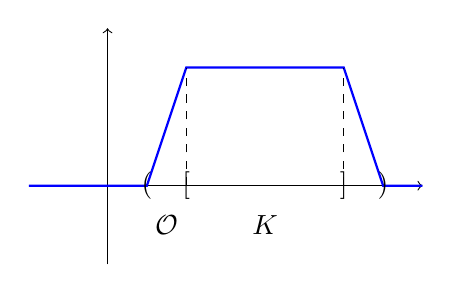
\begin{tikzpicture}
            \draw [->] (-1,0) -- (4,0);
            \draw [->] (0,-1) -- (0,2);
            \node at (1,0) {$[$};
            \node at (3,0) {$]$};
            \node at (2,-0.5) {$K$};
            %\draw [thick, decoration = {brace, mirror, raise = 0.5cm}, decorate] (1,0) -- (3,0);
            \draw [blue, thick] (-1,0) -- (0.5,0) -- (1,1.5) -- (3,1.5) -- (3.5,0) -- (4,0);
            \node at (0.5,0) {$($};
            \node at (3.5,0) {$)$};
            \node at (0.75,-0.5) {$\mathcal{O}$};
            \draw [dashed] (1,0) -- (1,1.5);
            \draw [dashed] (3,0) -- (3,1.5);
        \end{tikzpicture}
        \caption{Function given in \eqref{eq:function_in_r}.}
    \end{figure}
\end{frame}

\begin{frame}\frametitle{{\normalsize \secname} \\ {\large \subsecname}}
    The first to properties follows immediately, so we are left to show continuity.
    We have that
    \begin{align}
        \forall z \in E \, : \, \text{dist}(x, E) \leq |x-z|\leq |x-y|+|y-z|.
    \end{align}
    Taking the $\inf$ over $E \in Z$ yields
    \begin{align}
        \text{dist}(x, E)\leq |x-y|+\text{dist}(y, E),
    \end{align}
    the reverse inequality is obtained in the same way
    \begin{align}
        \text{dist}(y, E)\leq |x-y|+\text{dist}(x, E).
    \end{align}
\end{frame}

\begin{frame}\frametitle{{\normalsize \secname} \\ {\large \subsecname}}
    Thus we see that
    \begin{align*}
        |\text{dist}(x, E)-\text{dist}(y, E)|\leq |x-y|,
    \end{align*}
    which gives the continuity of the $\dist$ function, which makes $f_i$ a composition of continuous function and thus it is continuous.
    Furthermore the denominator cannot be zero.
\end{frame}

\begin{frame}\frametitle{{\normalsize \secname} \\ {\large \subsecname}}
    We can now $\forall \, K_i$ construct $f_i$.
    Lets now define the function
    \begin{align}
        F = \sum a_i f_i.
    \end{align}
    Using the triangular inequality on the $p$-norm of the difference between $\tilde{\varphi}$ and $F$ gives
    \begin{align}
        ||\tilde{\varphi}-F ||_p \ \leq  \sum |a_i| \, ||\chi_{K_i}-f_i ||_p.
    \end{align}
\end{frame}

\begin{frame}\frametitle{{\normalsize \secname} \\ {\large \subsecname}}
    The left part of the inequality (raised to the $p$-th power) satisfies
    \begin{align}
        ||\chi_{K_i} - f_i ||_p^p &= \int_{\mathbb{R}} | \chi_{K_i}(x) - f_i (x)|^p dx\\
         &= \int_{\mathcal{O}_i \backslash K_i} |f_i (x)|^p dx \\
         &\leq l^*(\mathcal{O}_i \backslash K_i) \\
         &\leq \left(\frac{\varepsilon}{\sum| a_i|}\right)^p,
    \end{align}
    this implies that
    \begin{align}
        ||\tilde{\varphi} - F||_p \leq \varepsilon.
    \end{align}
\end{frame}

\begin{frame}\frametitle{{\normalsize \secname} \\ {\large \subsecname}}
    We have now shown that we can ``approximate'' every simple function with compact support by a continuous function, which concludes the proof. \hfill $\square$
\end{frame}

\section{Fourier transform}

\subsection{Theorem 7.7}

\begin{frame}\frametitle{{\normalsize \secname} \\ {\large \subsecname}}
    \begin{theorem}[7.7]
        The Fourier transform is a linear bounded injective map from $L^1$ into $C_0$.
        Its inverse is given by
        \begin{align}\label{eq:rainbow_star}
            f(x) = \lim_{\varepsilon \rightarrow 0} \frac{1}{\sqrt{2 \pi}} \int_\mathbb{R} e^{ipx - \varepsilon |p|^2/2} \hat{f}(p) \, dp,
        \end{align}
        where the limit has to be understood in $L^1$.
        Moreover, this holds at every point of continuity.
    \end{theorem}
\end{frame}

\subsection{Proof of Theorem 7.7}

\begin{frame}\frametitle{{\normalsize \secname} \\ {\large \subsecname}}
    We know that the Fourier Transform is a function satisfying $F: L^1 (\mathbb{R}) \rightarrow C_0(\mathbb{R}) \subset C_b (\mathbb{R})$.
    $F$ is bounded since $\forall f \in L^1$
    \begin{align}
        \| F(f) \|_\infty \leq \frac{1}{2 \pi}\|f\|_1.
    \end{align}
    \vspace{1em}

    The first thing we will prove is that the Fourier Transform is injective, suppose therefore that we have already proved \eqref{eq:rainbow_star}.
\end{frame}

\begin{frame}\frametitle{{\normalsize \secname} \\ {\large \subsecname}}
    For $F$ to be injective, it means that
    \begin{align}
        f_1 \neq f_2 \ \Rightarrow \ F(f_1) \neq F(f_2).
    \end{align}
    We will use proof by contradiction, so assume that
    \begin{align}
        F(f_1) = F(f_2),
    \end{align}
    by linearity we have that
    \begin{align}
        F(f_1 - f_2) = F(f_1) - F(f_2) &= 0 \\
        \intertext{but this is also equal to}
        &= \widehat{(f_1 - f_2)}(p), \quad \forall \, p \in \hat{\mathbb{R}}.
    \end{align}
\end{frame}

\begin{frame}\frametitle{{\normalsize \secname} \\ {\large \subsecname}}
    As $f_1 - f_2 \in L^1(\mathbb{R})$, \eqref{eq:rainbow_star} gives that
    \begin{align}
        (f_1 - f_2)(x) = 0 \implies f_1 = f_2,
    \end{align}
    which is a contradiction.
    Thus we conclude that the Fourier Transform is an injective map.
    \vspace{1em}

    Next we can prove \eqref{eq:rainbow_star}.
\end{frame}

\begin{frame}\frametitle{{\normalsize \secname} \\ {\large \subsecname}}
    Let 
    \begin{align}
        \phi_\varepsilon(x) := \frac{1}{\sqrt{2 \pi}} e^{-\varepsilon \frac{|x|^2}{2}}
    \end{align}
    then we can rewrite the right hand side of \eqref{eq:rainbow_star} as
    \begin{align}
        \frac{1}{\sqrt{2 \pi}} \int_\mathbb{R} e^{ipx}e^{- \varepsilon |p|^2/2} \hat{f}(p) \, dp &= \int_\mathbb{R} e^{ipx} \phi_\varepsilon(p) \hat{f}(p) \, dp \\
        &= \frac{1}{\sqrt{2 \pi}} \int_\mathbb{R} \int_\mathbb{R} e^{ipx}  \phi_\varepsilon(p) e^{-ipy} f(y) \, dy \, dp.
    \end{align}
\end{frame}

\begin{frame}\frametitle{{\normalsize \secname} \\ {\large \subsecname}}
    By Tonelli's Theorem we have that the following inequality holds
    \begin{align}
        | e^{ipx}e^{-ipy} \phi_\varepsilon(p) f(y) | \leq \underbrace{|\phi_\varepsilon(p) |}_{\in \, L^1(\hat{\mathbb{R})}} \underbrace{| f(y) |}_{\in \, L^1(\mathbb{R})} \overbrace{\in}^{\text{Tonelli}} L^1( \mathbb{R} \times \mathbb{R}).
    \end{align}
    Applying now Fubini's Theorem gives
    \begin{align}
        \int_\mathbb{R} \widehat{\left( e^{ipx} \phi_\varepsilon  \right)}(y) f(y) \, dy &\overbrace{=}^{\text{Lemma 7.2 (2.)}} \int_\mathbb{R} \hat{\phi}_\varepsilon(y-x) f(y) \, dy \\
        &\overbrace{=}^{\text{Gaussian Lemma}} \int_\mathbb{R} \frac{1}{\sqrt{\varepsilon}} \phi_{\frac{1}{\varepsilon}}(y - x) f(y) \\ 
        &= (\Phi_\varepsilon * f)(x),
    \end{align}
\end{frame}

\begin{frame}\frametitle{{\normalsize \secname} \\ {\large \subsecname}}
    Where $\Phi_\varepsilon(x)$ is defined as
    \begin{align}
        \Phi_\varepsilon(x) := \frac{1}{\sqrt{2\pi}}\frac{1}{\sqrt{\varepsilon}}e^{-\frac{|x|^2}{2\varepsilon}},
    \end{align}
    where we have that $\Phi_\varepsilon(x)$ is an approximate identity, this means that
    \begin{align}
        \Phi_\varepsilon \geq 0, \ \Phi_\varepsilon \in C^\infty \text{ and }
        \int_\mathbb{R} \Phi_\varepsilon(x) dx = \underbrace{\frac{1}{\sqrt{2 \pi}} \int e^{-\frac{|x|^2}{2 \varepsilon}} dx}_{\text{Gaussian integral}} = 1
    \end{align}
\end{frame}

\begin{frame}\frametitle{{\normalsize \secname} \\ {\large \subsecname}}
    Taking now the limit as $\varepsilon$ goes to zero and using linear change of variable and the Dominated Convergence Theorem yields
    \begin{align}
        \forall r>0 \ \lim_{\varepsilon \rightarrow 0} \int_{|x| \geq r} \Phi_\varepsilon(x) \, dx = \lim_{\varepsilon \rightarrow 0} \int_{|x| \geq \frac{r}{\sqrt{\varepsilon}}} e^{-\frac{|x|^2}{2}} \, dx = 0
    \end{align}
    The right hand side thus becomes
    \begin{align}
        \lim_{\varepsilon \rightarrow 0} \Phi_\varepsilon * f = f,
    \end{align}
    by Lemma 3.19.
    This concludes the proof. \hfill $\square$
\end{frame}

\end{document}